\documentclass{article}

\usepackage[portuguese]{babel}
\usepackage[a4paper,top=2cm,bottom=2cm,left=3cm,right=3cm]{geometry}

\usepackage{amsmath}
\usepackage{graphicx}
\usepackage[colorlinks=true, allcolors=blue]{hyperref}
\usepackage{listings}
\usepackage{xcolor}
\usepackage{float}

\lstset{
    basicstyle=\ttfamily\small,
    backgroundcolor=\color{gray!10},
    frame=single,
    breaklines=true
}

\title{Projeto 2 de Segurança e Confiabilidade \\ Parte 2: Snort}
\author{
João Rodrigues 61789 \\
Rafael Figueiredo 61813 \\
Guilherme Sarreira 61860
}
\date{}

\begin{document}

\maketitle

\section{Introdução}

Nesta fase do projeto foi utilizado o sistema de deteção de intrusões \textit{Snort} com o objetivo de monitorizar o tráfego da máquina \textit{SperServ} e identificar comportamentos potencialmente maliciosos.

Foram desenvolvidas várias regras \textit{Snort} capazes de detetar diferentes tipos de ataques ou atividades suspeitas, nomeadamente:
\begin{itemize}
    \item varrimento de portos (\textit{port scanning});
    \item tentativas de descoberta de passwords;
    \item acessos externos não autorizados;
    \item possíveis ataques ICMP flood.
\end{itemize}

Neste relatório apresentam-se as regras implementadas, os métodos de teste utilizados e as evidências do correto funcionamento do sistema.

\section{Invocação do Snort}

Antes de executar o \textit{Snort} em modo de monitorização, foi utilizado o seguinte comando para verificar se o ficheiro de configuração não continha erros:

\begin{lstlisting}
sudo snort -T -c /etc/snort/snort.conf
\end{lstlisting}

A opção \texttt{-T} coloca o \textit{Snort} em modo de teste, validando a configuração e as regras definidas no ficheiro \texttt{snort.conf}.

Após a validação da configuração, o \textit{Snort} foi executado em modo consola através do comando:

\begin{lstlisting}
sudo snort -A console -q -c /etc/snort/snort.conf -i SperServ-eth0
\end{lstlisting}

Onde:
\begin{itemize}
    \item \texttt{-A console} apresenta os alertas diretamente na consola;
    \item \texttt{-q} executa o \textit{Snort} em modo silencioso;
    \item \texttt{-c} especifica o ficheiro de configuração utilizado;
    \item \texttt{-i SperServ-eth0} define a interface de rede monitorizada.
\end{itemize}

As regras desenvolvidas para deteção de ataques foram adicionadas ao ficheiro \texttt{local.rules}.

\section{Regras Snort Implementadas}

\subsection{Deteção de Port Scan}

Foi criada uma regra para detetar 20 ou mais ligações TCP provenientes da mesma máquina para portos inferiores a 1024 no intervalo de 60 segundos.

\begin{lstlisting}
alert tcp any any -> $HOME_NET 1:1023
(msg:"Port scan TCP (<1024)";
flags:S;
detection_filter:track by_src, count 20, seconds 60;
sid:1000001;
rev:1;)
\end{lstlisting}

Esta situação pode indicar uma tentativa de reconhecimento da máquina servidora através de \textit{port scanning}.

Para testar a regra foi utilizado o comando:

\begin{lstlisting}
nmap 10.0.0.2
\end{lstlisting}

Durante o teste o \textit{Snort} gerou o alerta esperado na consola.

\subsection{Deteção de Password Guessing}

Foi implementada uma regra para detetar 3 ligações TCP da mesma origem ao porto do \textit{SpertaServer} no intervalo de 20 segundos.

\begin{lstlisting}
alert tcp any any -> $HOME_NET 22345
(msg:"Tentativa de password guessing (3 ligacoes em 20s)";
flags:S;
detection_filter:track by_src, count 3, seconds 20;
priority:2;
sid:1000002;
rev:4;)
\end{lstlisting}

Este comportamento pode indicar uma tentativa de descoberta de passwords através de múltiplas ligações consecutivas.

Para testar a regra foi utilizado o comando:

\begin{lstlisting}
for i in 1 2 3; do
    nc -zv 10.0.0.2 22345
done
\end{lstlisting}

Após as três tentativas de ligação o alerta foi apresentado corretamente pelo \textit{Snort}.

\subsection{Deteção de Ligações Externas}

Foi criada uma regra para identificar tentativas de ligação provenientes de máquinas fora da sub-rede autorizada \texttt{10.0.1.0/24}.

\begin{lstlisting}
alert tcp !10.0.1.0/24 any -> $HOME_NET any
(msg:"Tentativa de acesso externo fora da sub-rede 10.0.1.0/24";
flags:S;
sid:1000003;
rev:1;)
\end{lstlisting}

Esta regra permite identificar acessos externos potencialmente não autorizados ao servidor.

Para testar a regra foi utilizado o comando:

\begin{lstlisting}
nc -zv 10.0.0.2 80
\end{lstlisting}

O \textit{Snort} gerou o alerta correspondente à tentativa de acesso fora da sub-rede autorizada.

\subsection{Deteção de ICMP Flood}

Foi implementada uma regra para detetar mais de 4 pedidos ICMP por segundo destinados ao servidor.

\begin{lstlisting}
alert icmp any any -> $HOME_NET any
(msg:"Possivel ICMP flood (>4 pings/s)";
itype:8;
detection_filter:track by_dst, count 4, seconds 1;
sid:1000004;
rev:1;)
\end{lstlisting}

Este tipo de tráfego pode indicar o início de um ataque de negação de serviço baseado em ICMP flood.

Para testar a regra foi utilizado o comando:

\begin{lstlisting}
sudo ping -i 0.1 10.0.0.2
\end{lstlisting}

Durante o teste foram gerados alertas indicando excesso de pedidos ICMP.

\section{Evidências (Screenshots/Prints)}

\begin{figure}[H]
    \centering
    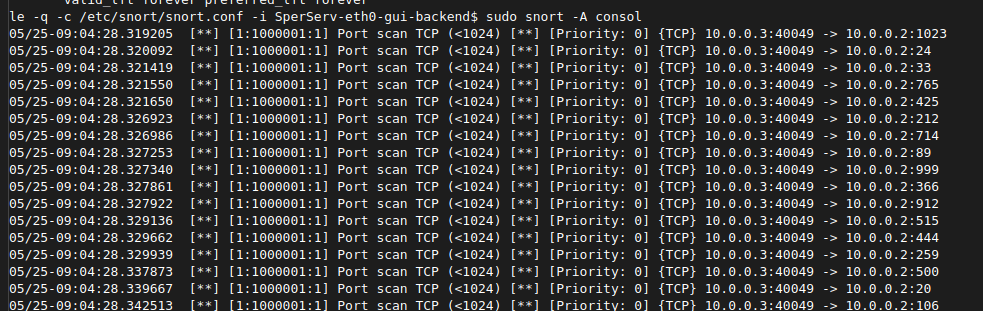
\includegraphics[width=0.60\linewidth]{image.png}
    \caption{Alerta gerado durante o teste de port scan com \texttt{nmap}.}
\end{figure}

\begin{figure}[H]
    \centering
    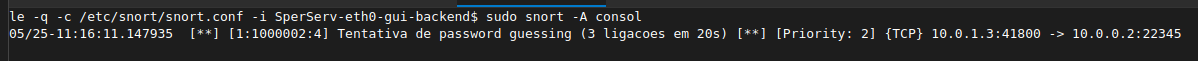
\includegraphics[width=0.60\linewidth]{segunda.png}
    \caption{Deteção de múltiplas ligações ao porto do SpertaServer.}
\end{figure}

\begin{figure}[H]
    \centering
    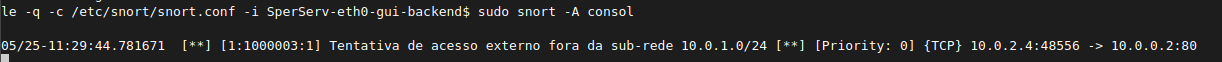
\includegraphics[width=0.60\linewidth]{3.png}
    \caption{Alerta de tentativa de acesso externo fora da sub-rede autorizada.}
\end{figure}

\begin{figure}[H]
    \centering
    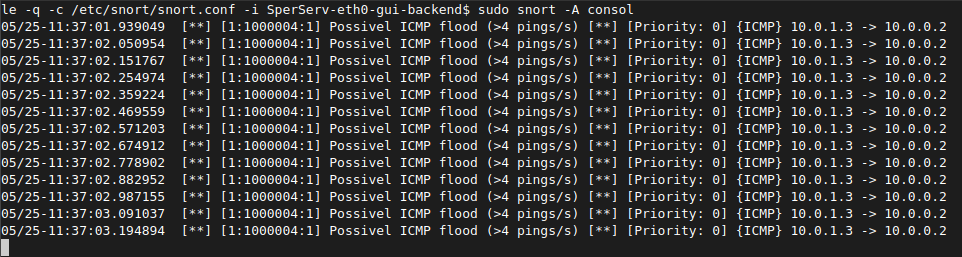
\includegraphics[width=0.60\linewidth]{4.png}
    \caption{Deteção de possível ataque ICMP flood.}
\end{figure}


\section{Observações e Dificuldades}

Durante a configuração do \textit{Snort} surgiram algumas dificuldades relacionadas com a definição correta das regras e dos parâmetros de deteção temporal.

Devido à versão do \textit{Snort} disponibilizada no ambiente \textit{Mininet}, não foi possível limitar corretamente a geração de alertas para apenas um alarme a cada 60 segundos na regra de deteção de \textit{port scan}. Apesar disso, a regra conseguiu detetar corretamente as tentativas de varrimento de portos.

Além disso, verificou-se que algumas regras apenas compilavam corretamente quando eram escritas integralmente numa única linha no ficheiro \texttt{local.rules}. Quando as regras eram divididas por várias linhas, o \textit{Snort} apresentava erros de parsing durante o carregamento da configuração.

Foi também necessário ajustar os testes para garantir que o número de ligações e os intervalos de tempo correspondiam exatamente às condições definidas nas regras.

Os testes realizados permitiram confirmar que o \textit{Snort} consegue identificar corretamente diferentes comportamentos suspeitos na rede, funcionando como um mecanismo complementar à firewall configurada anteriormente com \textit{iptables}.
\end{document}
sudo snort -T -c /etc/snort/snort.conf 

sudo snort -A console -q -c /etc/snort/snort.conf -i SperServ-eth0
